\documentclass[11pt,a4paper]{article}

\usepackage[margin=2.6cm]{geometry}
\usepackage{amsmath,amssymb}
\usepackage{graphicx}
\usepackage{booktabs}
\usepackage{array}
\usepackage{xcolor}
\usepackage{microtype}
\usepackage[font=small,labelfont=bf]{caption}
\usepackage[colorlinks=true,linkcolor=blue!50!black,citecolor=blue!50!black,urlcolor=blue!50!black]{hyperref}

\newcommand{\MP}{M_{\mathrm{P}}}
\newcommand{\TJ}{T_{J}}
\newcommand{\GeV}{\,\mathrm{GeV}}
\newcommand{\code}[1]{\texttt{#1}}

\title{The field equations in a Mathematica notebook and in the ChamPBH pipeline:\\
  an audit, and a comparison of histories with common thermodynamics}
\author{Prepared with Claude Code (Claude Opus 5.5) for D.~Seery}
\date{17 October 2026}

\begin{document}
\emergencystretch=3em
\maketitle

\begin{abstract}
\noindent
A companion report (\code{.documents/peakewsurf-kicking-function}) compared the kicking
function $\Sigma(\TJ) = 1 - 3w(\TJ)$ in the Mathematica notebook \code{PeakEWsurf.nb} with the
one in the ChamPBH pipeline. Here we check the rest of the system. We compare the field
equation term by term, together with the friction term, the law for the Jordan-frame
temperature, the radiation density, the matter fraction, the potential, the parameters and
the initial data. We then integrate the same histories with both codes, first giving both
the pipeline's thermodynamics and then giving both the notebook's.

\emph{The two codes solve the same system.} Mathematica's \code{Simplify} reduces the
difference between each code's field equation and the equation derived from the Friedmann and
Raychaudhuri equations to zero. The only structural difference is that the notebook computes
$\rho_r$ from $g_\rho(\TJ)\TJ^4$, while the pipeline integrates the continuity equation with
the tabulated $w$. These differ by up to $1.6\%$, because the table is not exactly
consistent with $g_\rho$ and $g_s$, but the difference has no effect on the field. In
this regime $V/\rho_r \le 10^{-49}$ and $f_m \le 4\times10^{-10}$, so the equations for $y =
\mathrm{d}\phi/\mathrm{d}N$ and $\ln\TJ$ depend only on $\Sigma(\TJ)$ and on $\gamma(\TJ) =
\mathrm{d}\ln g_s/3\,\mathrm{d}\ln\TJ$.

\emph{With common thermodynamics the histories agree to the accuracy of the integrators.}
With the pipeline's $\Sigma$, $\gamma$ and $f_m$ in both codes, the notebook's \code{NDSolve}
and the pipeline's Radau integrator agree to $|\Delta\ln\TJ| \le 7.5\times10^{-7}$ over
39 e-folds at all 13 couplings tested. The difference is the pipeline's own truncation error;
with its tolerance tightened to $10^{-10}$ it falls to $7\times10^{-9}$. Every $\TJ$ turning
point and every end point agrees, on both sides of both capture thresholds. Run the other way,
the pipeline's integrator reproduces the unmodified notebook to $3\times10^{-5}$. The two
integrators place each electroweak-capture threshold within the same $3\times10^{-7}$ in
$\beta$: $\beta_c \in (3.0028522, 3.0028525]$ with the notebook's thermodynamics and
$(3.0194601, 3.0194604]$ with the pipeline's.
Apart from $\Sigma$, the codes differ only through the notebook's $|\cdot|$ in the
temperature law. The Saikawa--Shirai fit has $\mathrm{d}g_s/\mathrm{d}T < 0$ between 0.7 and
3.5\,TeV, where the $|\cdot|$ delays the history by $3.2\times10^{-4}$ e-folds.

\emph{One result of the companion report is wrong.} The notebook's $\phi_i = 100\,\MP$
history is a numerical artefact. In the notebook, $\rho_r \propto (e^{\beta\phi}/\MP)^4$ is
formed in machine arithmetic and leaves the machine range once $\beta\phi \gtrsim 220$. The
true history does not depend on $\phi_i$, which only sets when $\phi$ reaches $0.1\,\MP$.
\end{abstract}

\tableofcontents

%======================================================================
\section{The two systems, term by term}
\label{sec:terms}

We use the notation of the companion report, with $\MP = 1$: $y = \mathrm{d}\phi/\mathrm{d}N$,
$N$ the Einstein-frame e-fold number, $A = e^{\beta\phi}$, $\rho$ the Einstein-frame
radiation density, $f = f_m = \rho_m/\rho$, $\Sigma = 1-3w$ and $D = \rho(1+f) + V$. The
notebook was read from its input cells by a Mathematica 15.0.1 kernel (SHA-256 in the
appendix); the pipeline from \code{ComputeTargets/ScalarModel.py} and
\code{ComputeTargets/Policies/PotentialDerivativePolicy.py} at commit \code{5ae2b65}.

\subsection{Field equation}

In e-folds the Klein--Gordon equation $\ddot\phi + 3H\dot\phi + V' = -\beta\rho(\Sigma+f)$
becomes
\begin{equation}
  y' = -\Bigl(3 + \frac{\dot H}{H^2}\Bigr) y - \frac{V' + \beta\rho(\Sigma + f)}{H^2},
  \qquad
  3H^2 = \frac{D}{1 - y^2/6},
  \qquad
  \dot H = -\tfrac12\bigl(\rho(1+w) + \rho f + H^2y^2\bigr).
  \label{eq:kg}
\end{equation}
The two codes split this as follows.
\begin{center}\footnotesize
\begin{tabular}{@{}lll@{}}
\toprule
Term & Notebook (cell 3) & Pipeline (\code{ODEPolicy}) \\
\midrule
force and kick & \code{rhsPhi}: $-3(1-\tfrac{y^2}{6})\dfrac{V' + \beta\rho(\Sigma+f)}{D}$ &
  $-V'/H^2 - 3E\beta\dfrac{\Sigma+f}{1+f}$, $E = 1-\tfrac{y^2}{6} - \tfrac{V}{3H^2}$ \\[2ex]
friction & $-(1-\tfrac{y^2}{6})\Bigl(1 + \dfrac{4V + (\Sigma+f)\rho}{2D}\Bigr)y$ &
  $-\bigl(G(1 + \tfrac R2) + \tfrac{V}{6H^2}(4-R)\bigr)y$, $G = 1-\tfrac{y^2}{6}$, $R = \tfrac{\Sigma+f}{1+f}$ \\
\bottomrule
\end{tabular}
\end{center}
\code{scripts/symbolic\_checks.wls} gives \code{Simplify} the difference between
Eq.~\eqref{eq:kg} and each code's right-hand side. Both differences reduce to $0$.

\subsection{Temperature, radiation and matter}

\paragraph{Jordan-frame temperature.} Both codes use entropy conservation in the Jordan frame,
\begin{equation}
  \frac{\mathrm{d}\ln\TJ}{\mathrm{d}N} = -\frac{1+\beta y}{1 + \gamma(\TJ)},
  \qquad
  \gamma = \frac{1}{3}\frac{\mathrm{d}\ln g_s}{\mathrm{d}\ln\TJ}.
  \label{eq:TJ}
\end{equation}
The notebook writes $\gamma = \tfrac13|\TJ g_s'/g_s|$. The pipeline has no $|\cdot|$. The two
agree only where $g_s$ increases with temperature (\S\ref{sec:thermo}).

\paragraph{Radiation density.} The notebook does not integrate $\rho$. It evaluates
$\rho = A^4(\pi^2/30)\,g_\rho(\TJ)\,\TJ^4$ at each step (\code{RhoRadA}). The pipeline
integrates $\mathrm{d}\ln\rho/\mathrm{d}N = \Sigma - 4 + \Sigma\beta y$, which is the
Jordan-frame continuity equation for the tabulated $w$ (checked symbolically, as is the
equation for $f$). Along a history, Eq.~\eqref{eq:TJ} gives $\mathrm{d}\ln\tilde\rho/\mathrm{d}\ln\TJ
= (4-\Sigma)(1+\gamma)$ for the Jordan-frame density $\tilde\rho = A^{-4}\rho$, which depends
on $\TJ$ alone. So the pipeline's $\tilde\rho$ is a function of $\TJ$, path-independent even
for histories that turn round, and differs from the notebook's by
\begin{equation}
  \Delta(\TJ) \equiv \ln\frac{\tilde\rho_{\rm pipe}}{(\pi^2/30)g_\rho\TJ^4}
  = \int_{\ln\TJ}^{\ln T_i}\Bigl[\Bigl(4 + \frac{\mathrm{d}\ln g_\rho}{\mathrm{d}\ln T}\Bigr)
     - (4-\Sigma)(1+\gamma)\Bigr]\mathrm{d}\ln T.
  \label{eq:delta}
\end{equation}
$\Delta$ vanishes if $w$, $g_\rho$ and $g_s$ are mutually consistent, since then $1 + w =
\tfrac43 g_s/g_\rho$ and $\mathrm{d}p/\mathrm{d}T = s$. The pipeline's table is not exactly
consistent with its $g_\rho$ and $g_s$. Starting at $T_i = 2\times10^4\GeV$, we find
$\Delta = +1.9\times10^{-3}$ at $100\GeV$ and $-1.6\times10^{-2}$ at $20\GeV$. It is
$-1.4\times10^{-2}$ at $1.64\GeV$ and $-2.1\times10^{-3}$ at $10\,\mathrm{MeV}$. With the
notebook's own table the values are similar, reaching $-1.8\times10^{-2}$ at $20\GeV$.

\paragraph{Matter fraction.} The notebook uses the closed form of the companion report
(\S3 there), with its $(1+w)$ inverted. The pipeline integrates $\mathrm{d}\ln
f/\mathrm{d}N = (1-\Sigma)(1+\beta y)$. By the argument above this makes $f$ a function of
$\TJ$ alone, $f = \rho_{m0}(1+z(\TJ))^3/\tilde\rho_{\rm pipe}(\TJ)$.

\subsection{Potential, coupling, parameters and initial data}

Both codes use $A = e^{\beta\phi/\MP}$ and $V = \Lambda^4 e^{M/\phi}$
(\code{ExponentialCoupling}, and \code{ExponentialPotential} with $n=1$). We give the pipeline
the notebook's parameters: $M = 10^{-2}\MP$, $\Lambda = 2.16\,\mathrm{meV}$ (the notebook's
$v_0 = 2.16\times10^{-12}\GeV/\MP$), $\phi_i = 10\,\MP$ and $y_i = 0$ at $T_i = 2\times10^4\GeV$.
At $T_i$ its initial $\rho$ is the notebook's $A^4(\pi^2/30)g_\rho\TJ^4$. The two Planck
masses differ, $2.43\times10^{18}\GeV$ in the notebook and $2.436\times10^{18}\GeV$ in the
pipeline. Since $\phi$ and $M$ are given in units of $\MP$ and $\Lambda$ and $\TJ$ in GeV,
only the ratios $V/\rho$ and $f$ enter Eq.~\eqref{eq:kg}, and $\MP$ cancels from both. The
notebook stops when $\phi$ falls to $0.1\,\MP$; the pipeline stops at a temperature. We
therefore integrate the pipeline beyond that point and cut its history where $\phi = 0.1\,\MP$
on its dense output.

\subsection{What the dynamics depends on}

Along every history integrated here, $V/\rho \le 10^{-49.7}$ and $f \le 4.3\times10^{-10}$.
The companion report also found $f/\Sigma \le 3.6\times10^{-4}$ wherever $\Sigma$ is
appreciable. To this accuracy Eq.~\eqref{eq:kg} becomes
\begin{equation}
  y' = -\Bigl(1-\frac{y^2}{6}\Bigr)\Bigl[3\beta\Sigma(\TJ) + \Bigl(1 + \frac{\Sigma(\TJ)}{2}\Bigr)y\Bigr],
  \label{eq:reduced}
\end{equation}
and together with Eq.~\eqref{eq:TJ} the pair $(y, \ln\TJ)$ evolves on its own. Neither $\phi$
nor the normalisation of $\rho$ appears. Two things follow.
\begin{enumerate}
\item $\Delta(\TJ)$, the matter fraction and the Planck mass all drop out of the dynamics here.
  The only inputs that can make the two codes' histories differ are $\Sigma(\TJ)$ and
  $\gamma(\TJ)$.
\item The history of $(y, \TJ)$ does not depend on $\phi_i$. A larger $\phi_i$ only lets the
  same history run for longer before $\phi$ reaches $0.1\,\MP$. Setting $V = 0$ in the notebook
  (variant \code{commonV0}) changes its $\beta = 3.015$ history by less than $10^{-12}$ in
  $\ln\TJ$.
\end{enumerate}

\medskip\noindent
\textbf{Conclusion 1.} \emph{The notebook and the pipeline integrate the same equations. In
the regime of these runs they differ only through the functions $\Sigma(\TJ)$ and
$\gamma(\TJ)$ they are given.}

%======================================================================
\section{The thermodynamic inputs}
\label{sec:thermo}

Both codes take $g_\rho$ and $g_s$ from the Saikawa--Shirai fits (arXiv:1803.01038,
App.~C), with identical coefficients. The notebook interpolates them linearly in $T$ on a
$10^{-4}$-dex grid. The pipeline splines them at 250 points per decade. The companion report
compared their $\Sigma$. Here we compare the other inputs, on a grid of 2000 points per decade
from $10^{-5}$ to $2\times10^4\GeV$ (\code{scripts/thermo\_compare.py},
\code{data/logs/thermo\_compare.txt}).
\begin{itemize}
\item $g_\rho$ and $g_s$ agree to $2.0\times10^{-4}$ and $3.5\times10^{-4}$. Both maxima
  are at $0.12\GeV$, where the fit switches between its low- and high-temperature branches,
  which do not quite meet.
\item $\gamma$ agrees to $2.4\times10^{-6}$ between 2 and $20\GeV$, and to $1.2\times10^{-5}$
  below $1\,\mathrm{MeV}$. Near the branch join at $0.12\GeV$ the two differ by up to
  $0.016$ in a narrow band, because the codes smooth the join differently.
\item \emph{The fitted $g_s$ falls with temperature between 702 and $3548\GeV$}, in both
  codes. The fit is not monotonic there; in the Standard Model $g_s$ is. In that band
  $\mathrm{d}g_s/\mathrm{d}\ln T$ reaches $-0.049$, so the notebook's $|\cdot|$ gives $\gamma$
  the wrong sign there, a change of up to $3.1\times10^{-4}$.
\end{itemize}
At a fixed Jordan-frame e-fold number $N_J$ ($\mathrm{d}N_J = (1+\beta y)\,\mathrm{d}N$), a change
$\delta\gamma$ shifts $\ln\TJ$ by $\int\delta\gamma\,\mathrm{d}\ln T/(1+\gamma)$, since
$\mathrm{d}\ln\TJ/\mathrm{d}N_J = -1/(1+\gamma)$.
Between $1.64\GeV$ and $T_i$ the notebook's $\gamma$ gives a total shift of $+3.15\times10^{-4}$
relative to the pipeline's. The $|\cdot|$ accounts for $+3.21\times10^{-4}$ of this, and the
difference in interpolation for $-3.5\times10^{-6}$. The branch join at $0.12\GeV$ would add
$1.1\times10^{-4}$, but no history here gets that cold. In the Einstein-frame histories the shift
appears as a delay: $|\Delta\ln\TJ|$ reaches $3.2\times10^{-4}$ where $\TJ$ falls freely and is
smaller while it surfs.

%======================================================================
\section{Histories with common thermodynamics}
\label{sec:runs}

\subsection{Method}

\paragraph{Notebook.} \code{scripts/nb\_common.wls} evaluates input cells 1--3 and runs the
notebook's \code{NDSolve} with its own options (\code{StiffnessSwitching}, accuracy and precision
goals 10, \code{MaxStepSize} $10^{-3}$, stop at $\phi = 0.1\,\MP$). Only the thermodynamic
inputs are changed:
\begin{center}\small
\begin{tabular}{@{}ll@{}}
\toprule
\code{nb} & unchanged: the notebook's $\Sigma$, $\gamma$ (with $|\cdot|$) and $f_m$ \\
\code{pipeSig} & the pipeline's $\Sigma$, the notebook's $\gamma$ and $f_m$ (the companion report's variant \code{pipe}) \\
\code{common} & the pipeline's $\Sigma$, $\gamma$ and $f_m(\TJ)$ \\
\bottomrule
\end{tabular}
\end{center}
The pipeline's functions were evaluated by its own code at 2000 points per decade and passed to
\code{NDSolve} as cubic interpolants in $\ln\TJ$. The variant \code{nb} keeps the notebook's
$\gamma$ inline in the $\TJ$ equation, exactly as the notebook does.

\paragraph{Pipeline.} \code{scripts/pipe\_runs.py} runs the pipeline's own \code{ODEPolicy},
\code{ODERHS} and \code{integrate\_scalar\_history}, the code path used in production, with
its default step control ($\mathrm{rtol} = \mathrm{atol} = 10^{-8}$). It builds the
initial state as \code{compute\_scalar\_model} does. It needs neither Ray nor a datastore; this
venv lacks \code{datastorekit}, which is replaced by a one-class stub (\code{scripts/dkstub.py}).
The cosmology is \code{QCD\_Cosmology} with \code{Planck2018}, the production configuration
(variant \code{pipe}). In variant \code{nbexact} it is wrapped so that it returns the
notebook's functions instead:
$\Sigma$ from 20\,000 samples per decade of the notebook's own interpolant, and $\gamma$
reproduced exactly from the nodes of the notebook's linear $g_s$ interpolant, with its
$|\cdot|$.

\paragraph{Couplings.} Thirteen values: the companion report's nine ($2.990$--$3.030$) and a
pair straddling each threshold ($3.0028$, $3.0029$; $3.0194$, $3.0195$).

\subsection{Results}

\begin{table}[ht]
\centering\footnotesize
\begin{tabular}{@{}c@{\hspace{1em}}lrr@{\hspace{1.5em}}lrr@{}}
\toprule
 & \multicolumn{3}{c}{Notebook's thermodynamics} & \multicolumn{3}{c}{Pipeline's thermodynamics} \\
\cmidrule(lr){2-4}\cmidrule(l){5-7}
$\beta$ & first min & $N$ (nb / pipe) & $N_{\rm end}$ & first min & $N$ (nb / pipe) & $N_{\rm end}$ \\
\midrule
2.9900 & QCD $1.6257$ & 29.16196 / 29.16193 & 38.93334 & QCD $1.6257$ & 22.911205 / 22.911204 & 38.93343 \\
2.9950 & QCD $1.6308$ & 32.86851 / 32.86848 & 38.98169 & QCD $1.6307$ & 23.808185 / 23.808184 & 38.97972 \\
3.0000 & none & -- & 36.5567 & QCD $1.6357$ & 24.972510 / 24.972510 & 39.02598 \\
3.0028 & none & -- & 35.74573 & QCD $1.6385$ & 25.802463 / 25.802462 & 39.05177 \\
3.0029 & EW $50.880$ & 14.6017 / 14.6010 & 35.74044 & QCD $1.6386$ & 25.835263 / 25.835263 & 39.05268 \\
3.0050 & EW $51.315$ & 11.30190 / 11.30190 & 35.67820 & QCD $1.6407$ & 26.586612 / 26.586612 & 39.07184 \\
3.0100 & EW $52.057$ & 10.28088 / 10.28088 & 35.65433 & QCD $1.6457$ & 29.092004 / 29.092004 & 39.11759 \\
3.0150 & EW $52.681$ & 9.83646 / 9.83646 & 35.66998 & QCD $1.6508$ & 34.083555 / 34.083554 & 39.15223 \\
3.0194 & EW $53.179$ & 9.57929 / 9.57929 & 35.69265 & none & -- & 35.94865 \\
3.0195 & EW $53.190$ & 9.57429 / 9.57429 & 35.69322 & EW $49.231$ & 14.51178 / 14.51177 & 35.93766 \\
3.0200 & EW $53.244$ & 9.54975 / 9.54975 & 35.69608 & EW $49.357$ & 12.368522 / 12.368522 & 35.89539 \\
3.0250 & EW $53.768$ & 9.33802 / 9.33802 & 35.72657 & EW $50.153$ & 10.478769 / 10.478769 & 35.82252 \\
3.0300 & EW $54.264$ & 9.17021 / 9.17021 & 35.75948 & EW $50.768$ & 9.966599 / 9.966599 & 35.84837 \\
\bottomrule
\end{tabular}
\caption{The first $\TJ$ minimum (in GeV) and the e-fold at which each code finds it, from
the notebook (\code{nb} and \code{common}) and the pipeline (\code{nbexact} and \code{pipe}).
$N_{\rm end}$, where $\phi = 0.1\,\MP$, agrees in every row to the digits shown; the largest
difference is $4.4\times10^{-5}$, at $\beta = 3.000$ with the notebook's thermodynamics.
``none'' means no minimum before $N_{\rm end}$. The minimum temperatures agree to
$6\times10^{-7}$ (left) and $6\times10^{-9}$ (right) in $\ln\TJ$.}
\label{tab:scan}
\end{table}

\begin{figure}[p]
\centering
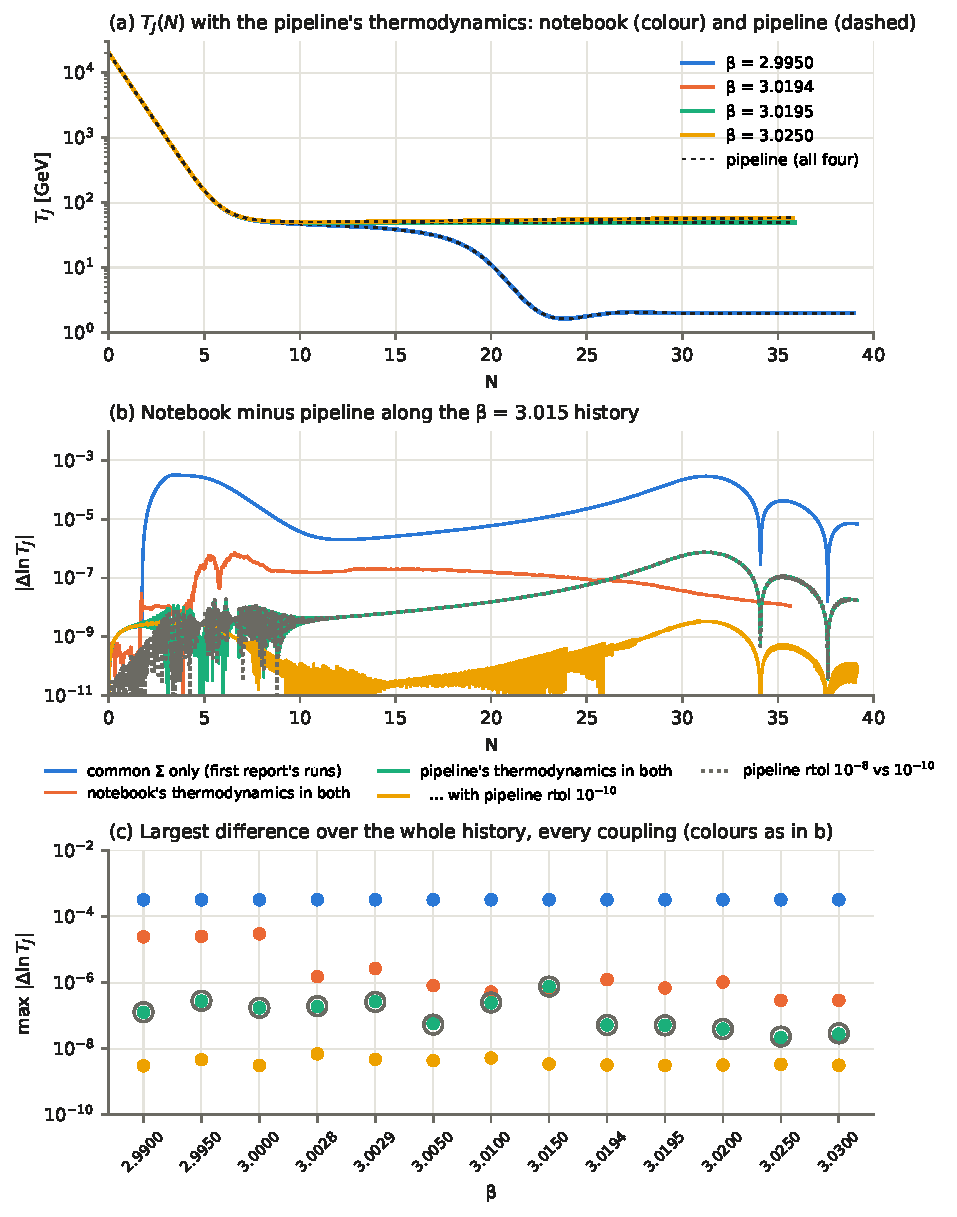
\includegraphics[width=\textwidth]{figures/agreement.pdf}
\caption{(a)~$\TJ(N)$ with the pipeline's thermodynamics, from the notebook (colour) and the
pipeline (dashed, drawn over each). $\beta = 3.0194$ and $3.0195$ lie either side of the
electroweak-capture threshold. (b)~The difference in $\ln\TJ$ along the $\beta = 3.015$ history
for each pairing. The dotted curve is the pipeline against itself at tolerances $10^{-8}$ and
$10^{-10}$. (c)~The largest difference over each whole history. Open markers are the dotted
pairing of panel (b); they ring the green markers, which they coincide with.}
\label{fig:agree}
\end{figure}

Table~\ref{tab:scan} and Fig.~\ref{fig:agree} give the results.
\begin{itemize}
\item \textbf{Pipeline's thermodynamics in both.} The notebook (\code{common}) and the pipeline
  (\code{pipe}) agree to $|\Delta\ln\TJ| \le 7.5\times10^{-7}$, $|\Delta\phi| \le 2.5\times10^{-7}$
  and $|\Delta y| \le 1.3\times10^{-7}$ at every coupling. Every turning point appears in both,
  in the same order, at the same $N$ to $10^{-6}$ ($9\times10^{-6}$ at $\beta = 3.0195$, the
  coupling closest to its threshold). This difference is exactly the pipeline's own truncation
  error: rerunning the pipeline at $\mathrm{rtol} = 10^{-10}$ changes it by the same
  $7.6\times10^{-7}$. At that tolerance it lies within $7\times10^{-9}$ of the notebook in
  $\ln\TJ$ and $2\times10^{-9}$ in $\phi$, at every coupling (Fig.~\ref{fig:agree}b, c).
\item \textbf{Notebook's thermodynamics in both.} The pipeline (\code{nbexact}) reproduces the
  unmodified notebook to $|\Delta\ln\TJ| \le 3.0\times10^{-6}$ for the histories captured at the
  electroweak scale. For those that reach the QCD transition ($\beta \le 3.000$) the bound is
  $3.0\times10^{-5}$. In this pairing the notebook's $\gamma$ is piecewise constant on
  $10^{-4}$-dex cells, so both integrators step across roughly $10^4$ discontinuities per
  decade of temperature. That is the most likely source of the larger residual; we did not
  separate it further. Resampling the notebook's functions at 2000 points per decade instead
  (variant \code{nbthermo}) gives $6\times10^{-4}$, so the sampling must be fine.
\item \textbf{Common $\Sigma$ only.} The companion report's runs (\code{pipeSig}) differ from
  the pipeline by up to $3.2\times10^{-4}$ in $\ln\TJ$ at every coupling. This is a delay of
  $3.2\times10^{-4}$ e-folds, seen in full where $\TJ$ falls freely and less while it surfs
  (Fig.~\ref{fig:agree}b); the end points move by the same $3.2\times10^{-4}$. It comes from the
  notebook's $|\cdot|$ (\S\ref{sec:thermo}), and it is dynamically negligible.
\end{itemize}

\paragraph{The thresholds.} We bisected with the pipeline's integrator to a tolerance of
$10^{-6}$ in $\beta$ (\code{data/logs/pipeline\_bisections.txt}). We then ran the notebook at
five couplings across each pipeline bracket (\code{data/logs/notebook\_thrnb\_log.txt},
\code{notebook\_thrcommon\_log.txt}). Each row uses one set of thermodynamics in both codes.
\begin{center}\small
\begin{tabular}{@{}llll@{}}
\toprule
Thermodynamics & Pipeline integrator & Notebook integrator & Notebook (companion report) \\
\midrule
notebook's & $(3.0028522,\ 3.0028528]$ & $(3.0028522,\ 3.0028525]$ & $(3.002813,\ 3.002891)$ \\
pipeline's & $(3.0194598,\ 3.0194604]$ & $(3.0194601,\ 3.0194604]$ & $(3.019453,\ 3.019531)$ \\
\bottomrule
\end{tabular}
\end{center}
The two integrators place each threshold within the same $3\times10^{-7}$ in $\beta$. The
pipeline brackets are unchanged at $\mathrm{rtol} = 10^{-10}$, and unchanged when the
notebook's $\Sigma$ is used with either code's $\gamma$ (variants \code{nbsig},
\code{nbthermo} and \code{nbexact}). The companion report's column used the notebook's
$\gamma$ and $f_m$ throughout. The pipeline's own fine scan near $\beta = 3$ places its edge
in $(3.019, 3.020]$. That scan used another potential and $\phi_i$, and its own classification
of capture; neither the potential nor $\phi_i$ enters the $(y, \TJ)$ equations here
(\S\ref{sec:terms}), so the agreement is expected.

\medskip\noindent
\textbf{Conclusion 2.} \emph{Given the same $\Sigma$ and $\gamma$, the notebook and the
pipeline yield the same field histories to the accuracy of their integrators, and the same
capture thresholds. Every difference between them traced so far comes from $\Sigma$
(companion report) or, at the level of $3\times10^{-4}$ in $\ln\TJ$, from the notebook's
$|\cdot|$.}

%======================================================================
\section{Large initial fields: machine overflow in the notebook}
\label{sec:overflow}

By \S\ref{sec:terms} the $(y, \TJ)$ history does not depend on $\phi_i$. The pipeline confirms
this: at $\beta = 3.005$ its $\phi_i = 10$, 50, 58, 60 and $100\,\MP$ histories have the same
turning points to all digits printed. The notebook does too, up to $\phi_i = 72\,\MP$: its
$\phi_i = 50$, 58, 60, 66, 68, 70 and $72\,\MP$ histories reproduce its $\phi_i = 10\,\MP$ one to
$|\Delta\ln\TJ| \le 2.5\times10^{-6}$, most of them to $10^{-9}$. At $\phi_i = 75$ and $100\,\MP$ they do not (Fig.~\ref{fig:overflow}).

\paragraph{Cause.} The notebook evaluates $\rho = (A/\MP)^4(\pi^2/30)g_\rho\TJ^4$ with
$A = e^{\beta\phi}$ (\code{RhoRadA}), and $(A/\MP)^4$ exceeds the largest machine number,
$1.8\times10^{308}$, once $\beta\phi > \ln(1.16\times10^{77}\times2.43\times10^{18}) = 219.8$:
at $\phi = 73.1\,\MP$ for $\beta = 3.005$. The sweep brackets the onset between $\beta\phi_i =
216.4$ (correct) and $225.4$ (wrong), consistent with this. Mathematica then switches silently to
arbitrary-precision numbers (the integrations run under \code{Quiet}), and some combinations
underflow: in machine arithmetic $0.03\times(4.0\times10^{457})^{-1}$ returns $0$ with a
\code{General::munfl} message. Evaluated one point at a time, the notebook's right-hand side is
still exactly the same at $\phi = 10$ and $100\,\MP$. Inside \code{NDSolve}, however, one e-fold
from $y = -0.05$, $\TJ = 200\GeV$ gives $y = -0.148691$ from $\phi = 10$ or $50\,\MP$ but
$-0.149436$ from $\phi = 100\,\MP$. We did not identify which internal evaluation goes wrong.
The error persists for as long as $\phi \gtrsim 73\,\MP$, that is until $N \approx 87$ for
$\phi_i = 100$. The spurious $\TJ$ maximum the companion report found at $N = 82.95$ (where
$\phi = 74.3\,\MP$) belongs to the end of this stretch.

\paragraph{Check.} \code{nb\_common.wls} has log-space variants (suffix \code{Log}) with the
numerator and denominator of the right-hand side divided by $\rho$, and $V/\rho$ formed from
logarithms. The pipeline computes $V/3H^2$ the same way. The change is algebraically
nothing, and at $\phi_i = 10$ it reproduces the notebook to ten digits. At $\phi_i = 100\,\MP$
the log-space notebook agrees with the pipeline over all 150 e-folds, to $|\Delta\ln\TJ| \le
8\times10^{-7}$ with the notebook's thermodynamics and $3\times10^{-8}$ with the pipeline's
(Fig.~\ref{fig:overflow}). With the notebook's
thermodynamics, $\TJ$ has a single minimum at $N = 11.30$ ($51.31\GeV$), the same as for
$\phi_i = 10$, then rises slowly to $58.36\GeV$ at $N = 150$. With the pipeline's, the history
is captured at the QCD transition at $N = 26.59$ ($1.641\GeV$), as for $\phi_i = 10$, and
oscillates about $1.992\GeV$.

\begin{figure}[ht]
\centering
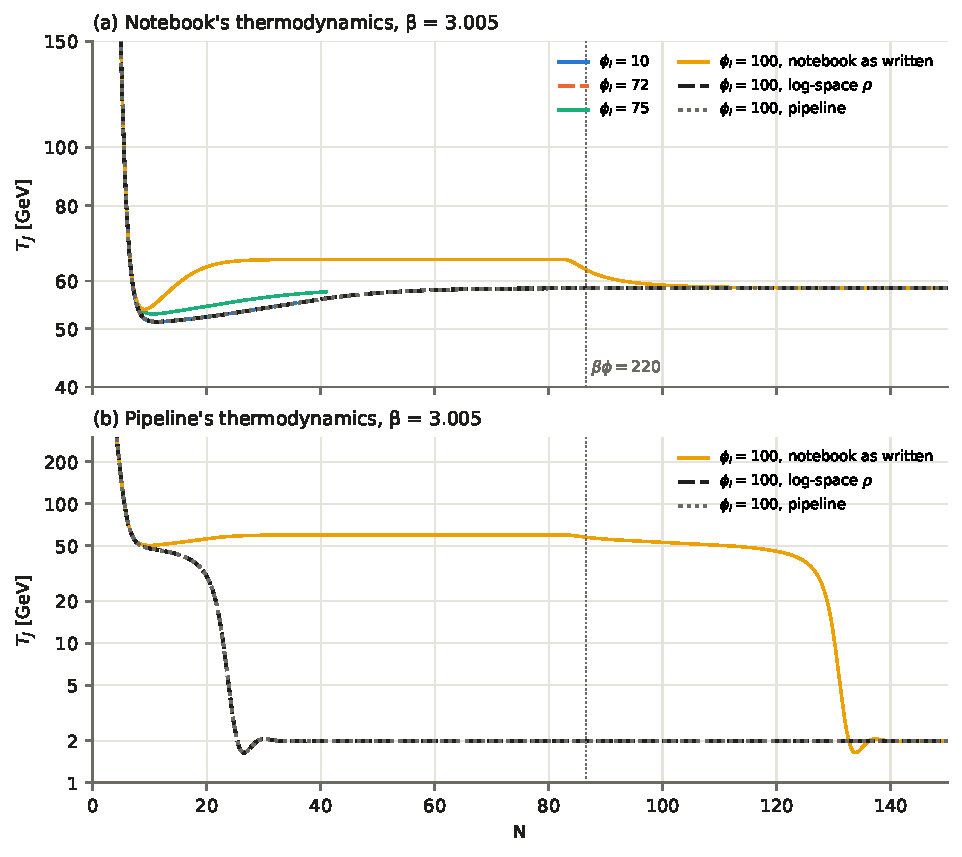
\includegraphics[width=\textwidth]{figures/overflow.pdf}
\caption{$\TJ(N)$ at $\beta = 3.005$. (a)~The notebook's thermodynamics: the notebook at
$\phi_i = 10$, 72, 75 and $100\,\MP$, the log-space notebook at $100\,\MP$, and the pipeline at
$100\,\MP$. The $\phi_i \le 72$ curves, the log-space curve and the pipeline's lie on top of
one another. (b)~The pipeline's thermodynamics at $\phi_i = 100\,\MP$. The dotted line marks
where the $\phi_i = 100\,\MP$ history falls back through $\beta\phi = 220$.}
\label{fig:overflow}
\end{figure}

\paragraph{Consequences.}
\begin{enumerate}
\item \emph{The companion report's ``longer history'' (its \S4.2 and Fig.~5) is an artefact.}
  The true $\phi_i = 100\,\MP$ histories are those just described, not an electroweak minimum
  at $N \approx 9$--$10$ for both $\Sigma$ followed by a maximum at $N \approx 83$. Its other
  results use $\phi_i = 10\,\MP$ ($\beta\phi \le 30.3$) and stand.
\item The notebook's own $\phi_i = 100\,\MP$ cells are affected in the same way. These are
  cells 10--11 ($\beta = 3.005$) and cell 16 ($\beta = 2.35$, $\beta\phi_i = 235$), and with them
  the plots drawn from those solutions (cells 12--15 and 17--22).
\end{enumerate}

%======================================================================
\section{The matter fraction at late times}
\label{sec:fmlate}

The companion report found that the notebook's closed-form matter fraction has its $(1+w)$
dependence inverted (its \S3), and that this has no effect on the dynamics near $\beta = 3$. One
might expect the error to matter at late times, when matter comes to dominate and the kick
$\propto \beta(\Sigma + f_m)/(1+f_m)$ is carried by $f_m$ alone. It does not, for the two reasons
below. A different simplification in the same formula does matter at late times, however.
\code{scripts/nb\_fm\_late.wls} exports the notebook's $f_m$ and $w$ down to $T_{\rm CMB}$, and
\code{scripts/fm\_late.py} compares them with the pipeline's $f_m(\TJ) = \rho_{m0}(1+z)^3/\tilde\rho$
(\S\ref{sec:terms}). The results are in \code{data/fm\_late.csv} and \code{data/logs/fm\_late.txt}.

\paragraph{The runs never reach the matter era.} Every history here ends when $\phi$ reaches
$0.1\,\MP$, at $N \approx 36$--$39$ and $\TJ$ between $1.6$ and $60\GeV$. There $f_m \le
4\times10^{-10}$, against $\Sigma \approx 0.03$--$0.3$ at the peaks. Matter--radiation
equality is at $\TJ \approx 0.80\,\mathrm{eV}$, twenty or more e-folds further on, and no run in
either report integrates that far. Whatever form $f_m$ takes, it cannot affect these histories.

\paragraph{The $(1+w)$ error vanishes where $w = 1/3$.} The notebook uses
\begin{equation}
  f_m^{\rm nb} = \frac{4}{3}\,\frac{c}{\TJ\,(1+w)}, \qquad c = 5.213\times10^{-10}\GeV,
\end{equation}
whereas for a plasma at a single temperature $\tilde\rho + \tilde p = \TJ s$, which gives
$f_m = (\rho_m/s)(1+w)/\TJ$. The notebook's form is therefore larger by $(16/9)/(1+w)^2$, a
factor that is exactly $1$ at $w = 1/3$. It departs from $1$ only where $w$ does: by up to
$1.178$ at the QCD peak, $1.05$ at the $e^\pm$ peak and $1.02$ at the electroweak peak
(Fig.~\ref{fig:fmlate}). At those peaks $\Sigma$ exceeds $f_m$ by about $2\times10^4$ ($e^\pm$), $7\times10^7$ (QCD) and
$3\times10^9$ (electroweak).
Below $36\,\mathrm{keV}$ the notebook sets $w = 1/3$ exactly, so the factor is exactly $1$
throughout the matter era.

\paragraph{What does matter late: $g_s \ne g_\rho$.} The relation $\tilde\rho + \tilde p = \TJ s$
holds only while the whole plasma shares one temperature. After neutrino decoupling and $e^\pm$
annihilation the photons and neutrinos have different temperatures, and the correct late-time
result is
\begin{equation}
  f_m = \frac{\rho_m}{s}\,\frac43\,\frac{g_s}{g_\rho}\,\frac{1}{\TJ},
  \qquad \frac{g_s}{g_\rho} = \frac{3.931}{3.383} = 1.1620.
\end{equation}
The notebook's formula effectively sets $g_s = g_\rho$. Below $10\,\mathrm{keV}$ the ratio of the
two codes' $f_m$ is therefore constant:
\begin{equation}
  \frac{f_m^{\rm nb}}{f_m^{\rm pipe}} = 0.8682
  = \underbrace{1}_{(1+w)} \times \underbrace{0.8606}_{g_\rho/g_s}
    \times \underbrace{1.0097}_{c/(\rho_m/s)_{\rm pipe}}
    \times \underbrace{0.9992}_{e^{\Delta}}.
\end{equation}
The third factor is the difference between the notebook's constant and $\rho_m/s =
5.163\times10^{-10}\GeV$ from the pipeline's Planck 2018 parameters. The fourth is the
pipeline's thermodynamic offset $\Delta$ (Eq.~\ref{eq:delta}), which is constant below
$10\,\mathrm{keV}$. This is the $0.87$ the companion report saw at $10\,\mathrm{keV}$, and it
persists to today. Between $10\,\mathrm{keV}$ and $1\,\mathrm{MeV}$, where $g_s/g_\rho$ is
changing, the ratio climbs to $1$ (Fig.~\ref{fig:fmlate}).

\begin{figure}[ht]
\centering
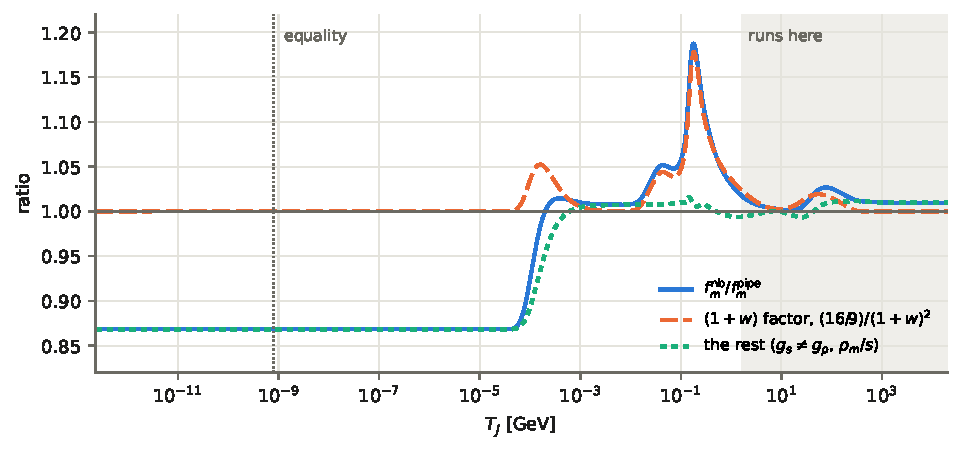
\includegraphics[width=\textwidth]{figures/fm_late.pdf}
\caption{The notebook's matter fraction relative to the pipeline's, from $T_{\rm CMB}$ to
$2\times10^4\GeV$ (solid), split into the notebook's $(1+w)$ factor (dashed) and everything else
(dotted). The shaded band is the range of $\TJ$ the histories of this report cover; the dotted
line is matter--radiation equality.}
\label{fig:fmlate}
\end{figure}

\paragraph{Consequence if the notebook were run to late times.} Its $f_m$ would be $13\%$ low
throughout the matter era. Equality, where $f_m = 1$, would fall at $\TJ = 0.695\,\mathrm{eV}$
instead of $0.800\,\mathrm{eV}$, that is $15\%$ later in the scale factor, or $0.14$ e-folds.
That would shift the onset of the matter-driven kick and the expansion rate around it. The error
comes from omitting $g_s \neq g_\rho$, not from the $(1+w)$ factor. Correcting only the $(1+w)$
placement would leave it unchanged. The pipeline is not affected: it integrates
$\mathrm{d}\ln f_m/\mathrm{d}N = (1-\Sigma)(1+\beta y)$, whose solution includes $g_s \ne g_\rho$
through $z(\TJ)$.

%======================================================================
\section{Observations not acted on}

\begin{itemize}
\item \textbf{The pipeline's $\rho_r$ is not $(\pi^2/30)g_\rho\TJ^4$.} Because the $w$ table is
  not exactly consistent with $g_\rho$ and $g_s$, the integrated $\tilde\rho$ differs from it by
  $\Delta(\TJ)$ (Eq.~\ref{eq:delta}), up to $1.6\%$ near $20\GeV$ for $T_i = 2\times10^4\GeV$.
  The field histories here do not depend on it. The pipeline's stored $\rho_r$ and $H$ do, and
  so would any regime in which $V/\rho_r$ is not negligible. Because $\Delta$ is a function of
  $\TJ$ and $T_i$ alone, it is easy to tabulate if needed.
\item \textbf{The Saikawa--Shirai $g_s$ fit is not monotonic} between 0.7 and $3.5\,\mathrm{TeV}$.
  The effect on these histories is $3\times10^{-4}$ in $\ln\TJ$.
\item \textbf{The venv has no \code{datastorekit}.} \code{requirements.txt} pins \code{v0.4.0},
  but \code{import datastorekit} fails in \code{./venv}, so as it stands the test suites cannot
  import \code{ComputeTargets.ScalarModel}. These runs used a stub.
\end{itemize}

%======================================================================
\section{Summary and recommendations}

\begin{enumerate}
\item The notebook and the pipeline integrate the same field equation, friction term and
  temperature law (\S\ref{sec:terms}). Their only structural difference, $\rho_r$ algebraic
  against integrated, has no effect on the field in this regime.
\item Given the same $\Sigma$ and $\gamma$ their histories agree to $7\times10^{-9}$ in
  $\ln\TJ$, and their capture thresholds agree to $3\times10^{-7}$ in $\beta$ (\S\ref{sec:runs}). The difference between
  the codes' published capture edges is therefore entirely the difference in $\Sigma$ that the
  companion report found.
\item Apart from $\Sigma$, the notebook differs only through its $|\cdot|$ in $\gamma$, which
  delays the histories by $3.2\times10^{-4}$ e-folds.
\item The notebook's $\phi_i = 100\,\MP$ results are corrupted by machine overflow
  (\S\ref{sec:overflow}).
\item The notebook's inverted $(1+w)$ factor in $f_m$ is harmless at every temperature: it is
  exactly $1$ wherever $w = 1/3$, including the whole matter era. Its $f_m$ is nonetheless $13\%$
  low after $e^\pm$ annihilation, because it omits $g_s \ne g_\rho$. No run here reaches the
  matter era, but a run that did would place equality $15\%$ late in the scale factor
  (\S\ref{sec:fmlate}).
\end{enumerate}

\noindent We recommend:
\begin{itemize}
\item In the notebook, form the right-hand side in terms of $V/\rho$ and $V'/\rho$ evaluated
  through logarithms, as the log-space variant does, or keep $\beta\phi < 220$. Remove the Quiet
  around \code{NDSolve}, or at least catch \code{General::ovfl} and \code{General::munfl}.
\item In the notebook, drop the $|\cdot|$ in $\gamma$, so that it matches the pipeline.
\item Before the notebook is run into the matter era, replace its closed-form $f_m$ with the
  pipeline's, $\rho_{m0}(1+z)^3/\tilde\rho_r$ (or integrate $\ln f_m$). Correcting only the $(1+w)$
  placement, as the companion report suggested, would leave the $13\%$ error.
\item Correct the companion report's \S4.2 and Fig.~5 with an additive note pointing here.
\end{itemize}

\paragraph{Not covered.} Integrations in regimes where $V/\rho_r$ or $f_m$ is not negligible
(late times, smaller $\phi$ near $M$, or the pipeline's reflections at the wall). There the
normalisation $\Delta(\TJ)$ and the matter fraction start to matter; \S\ref{sec:fmlate}
compares the two codes' $f_m$ there but integrates nothing. Temperatures below $0.12\GeV$, where
the two codes' $\gamma$ differ near the branch join. Couplings far from $\beta = 3$.

%======================================================================
\appendix
\section{Reproducing these results}

\paragraph{Versions.}
\begin{itemize}
\item Notebook \code{PeakEWsurf.nb}, not under version control, SHA-256\\
  {\small\code{5bd78e6f43b6b7fc4a2eaff746263b63a66c27786eef76cea90edbdd070e92e4}} (the same file
  as the companion report's).
\item ChamPBH at commit \code{5ae2b65}; Mathematica 15.0.1 (macOS, ARM); Python 3.13 with NumPy
  2.3.5 and SciPy 1.17.0.
\end{itemize}

\paragraph{Files.} Everything is in \code{.documents/peakewsurf-field-equations/}.
\begin{itemize}
\item \code{scripts/symbolic\_checks.wls}: the symbolic checks of \S\ref{sec:terms}.
\item \code{scripts/nb\_thermo.wls}, \code{nb\_export\_exact.wls}: export the notebook's
  thermodynamic functions; \code{thermo\_compare.py}: compares them with the pipeline's, computes
  $\Delta(\TJ)$ and writes the pipeline's functions for \code{nb\_common.wls}.
\item \code{scripts/nb\_fm\_late.wls}, \code{fm\_late.py}: the matter fraction down to
  $T_{\rm CMB}$ (\S\ref{sec:fmlate}); \code{fm\_late.py} reads \code{nb\_fm\_late.csv} and the
  \code{delta\_pipe.csv} that \code{thermo\_compare.py} writes.
\item \code{scripts/nb\_common.wls}: the notebook's integration with swapped inputs;
  \code{rhs\_phi\_dep.wls}: the overflow demonstration.
\item \code{scripts/pipe\_runs.py}, \code{bisect\_pipe.py}, \code{dkstub.py}: the pipeline's
  integrations and bisections.
\item \code{scripts/compare\_histories.py}, \code{build\_data.py}, \code{make\_figures.py}:
  the comparison, the data products and the figures.
\item \code{data/}: \code{compare.json} (every pairing, every coupling), \code{max\_residuals.csv},
  \code{pipeline\_runs.json} (every pipeline run's turning points), downsampled histories and
  residuals, and the logs of every notebook run, bisection and comparison.
\end{itemize}

\paragraph{Commands.} Run from the repository root, with \code{WORK} a scratch directory and
\code{WolframKernel} set as in the companion report.
{\small
\begin{verbatim}
D=.documents/peakewsurf-field-equations/scripts
wolframscript -file $D/nb_thermo.wls $PWD/PeakEWsurf.nb $WORK
wolframscript -file $D/nb_export_exact.wls $PWD/PeakEWsurf.nb $WORK
./venv/bin/python $D/thermo_compare.py $WORK
wolframscript -file $D/nb_fm_late.wls $PWD/PeakEWsurf.nb $WORK
./venv/bin/python $D/fm_late.py $WORK
export NB_THERMO_GRID=$WORK/nb_thermo_grid.csv NB_EXACT_DIR=$WORK
B=2.99,2.995,3.0,3.0028,3.0029,3.005,3.01,3.015
B=$B,3.0194,3.0195,3.02,3.025,3.03
for v in pipe nbexact nbthermo nbsig; do
  ./venv/bin/python $D/pipe_runs.py $WORK/pipe $B $v 10 41; done
./venv/bin/python $D/pipe_runs.py $WORK/pipe_r10 $B pipe 10 41 1e-10
./venv/bin/python $D/pipe_runs.py $WORK/pipe100 3.005 pipe 100 150   # and nbexact
wolframscript -file $D/nb_common.wls $PWD/PeakEWsurf.nb $WORK/nbrun \
    $WORK/pipe_thermo_grid.csv "{${B}}" '{"nb","pipeSig","common"}' \
    "10^-3" 10 150 scan True \
    > $WORK/nbrun/scan_log.txt
./venv/bin/python $D/bisect_pipe.py 2.995 3.005 nbexact 1e-6
./venv/bin/python $D/bisect_pipe.py 3.015 3.02 pipe 1e-6
\end{verbatim}
}
\noindent The $\phi_i$ sweep runs \code{nb\_common.wls} with $\phi_i \in \{50, 58, 60, 66, 68,
70, 72, 75\}$ (tags \code{phi}$\phi_i$ and \code{onset}$\phi_i$, $N_{\max} = 41$), and with
$\phi_i = 100$, $N_{\max} = 150$ for the variants \code{nb}, \code{common}, \code{nbLog} and
\code{commonLog} (tag \code{p100long}). The pipeline's $\phi_i = 50$, 58 and $60$ runs go to
\code{WORK/pipephi}$\phi_i$. The notebook threshold runs pass two more arguments, the decimals in
the file names and a time limit per run: \code{... "10\^{}-3" 10 150 thrnb True 7 240} with the
variant \code{"nb"}, and the same with \code{"common"} and tag \code{thrcommon}. Then \code{compare\_histories.py WORK},
\code{build\_data.py WORK} and \code{make\_figures.py}. A notebook integration takes
20--30\,s for \code{nb}, and 1--3\,min for the swapped variants, whose functions are evaluated
through \code{?NumericQ} wrappers. The log-space variants take longer still. A pipeline
integration takes under a second.

\end{document}
